\section{Experiments}
\label{sec:results}

We begin by describing the three datasets we will consider: a synthetic binary classification task,
and two real-world data sets in document classification and sequence tagging.
We then present our results.  We first show that active over-labeling
improves accuracy over standard active or passive learning. 
We then study how \sys 's 
performance varies with the relative labeling cost between
coarse (root) and fine (lower-level) labels and overall budget
(number of training examples).
Finally, we show how our adaptive bandit-based
over-labeling scheme, BANDIT, is robust
to changes in labeling cost and budget\footnote{The
code and dataset used in this experiment can be downloaded from
\url{http://github.com/moyuji/hal}}.

\subsection{Synthetic Dataset}
\label{sec:synth}

First we assess the advantage provided by using fine-grained label data in a synthetic binary
classification task. In this dataset the sole feature is a single continuous value
$x\in[0,18)$. The positive instances are all points in the $9$ level-3 intervals
$\{[0,1), [2,3), [4,5),\ldots,[16,17) \}$. We define the level-2 intervals by taking 
the union of consecutive triples of the level-3 intervals:
$\{[0,1), [2,3), [4,5) \}$, $\{[6,7), [8,9), [10,11) \}$, and
$\{[12,13), [14,15), [16,17) \}$. The level-1 label (positive versus negative) 
is the union of the three level-2 labels.
% (see~Figure~\ref{fig:hier-synth}). 
The goal is to learn the level-1 label of `$+$' versus `$-$'. 
We use as our base learner the Gradient Boosted Regression
Tree~(GBRT)~\cite{Friedman2001}, which is an ensemble of regression trees. 
We set the maximum depth in GBRT to be $1$ 
so that each tree maps to an interval. For the fine-grained learner,
the classifers at level 3 are combined with the level-2 classifier and then the
coarse-level classifier using Equation~\ref{eq:maxcombine}. Because GBRT can be
a union of intervals, the classifiers at each level should be expressive enough
to capture the target concept.


%%% SDS dropping this to save space
% \begin{figure}[h]
% \vskip 0.2in
% \begin{center}
% \centerline{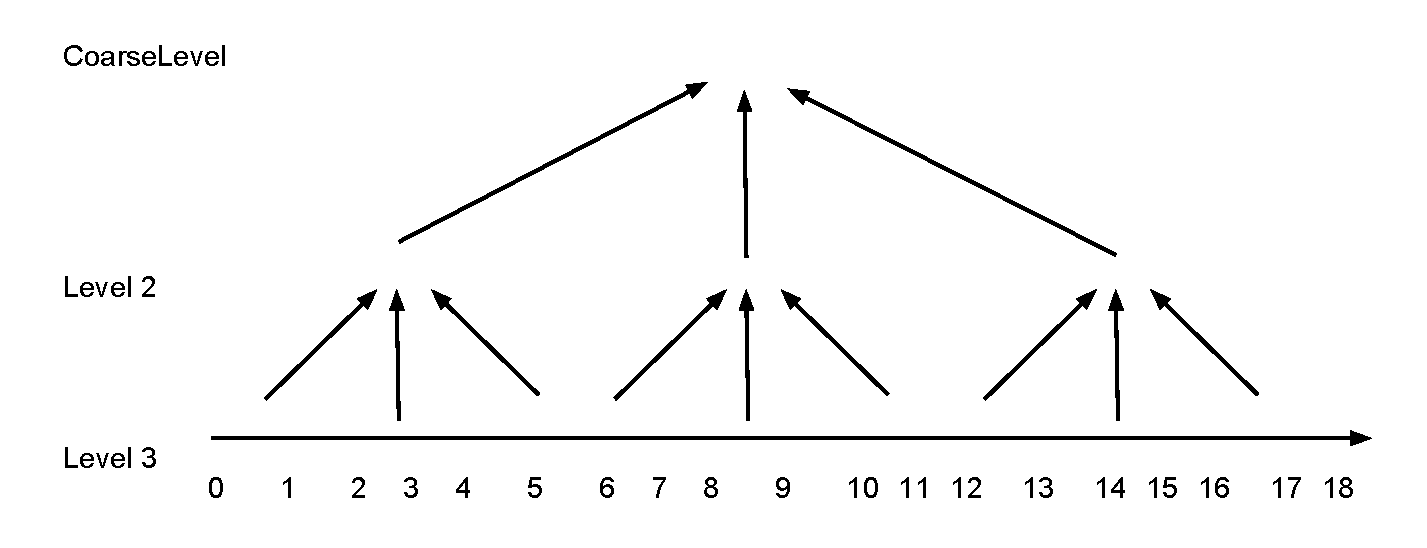
\includegraphics[width=\columnwidth]{fig/intervals.pdf}}
% \caption{The 3-level labeling  structure of the synthetic data set.}
% \label{fig:hier-synth}
% \end{center}
% \vskip -0.2in
% \end{figure} 

We chose $n=30$ trees, learning rate $\lambda=0.9$ and sample rate $r=0.8$ for our GBRT
learners.  Learners started with $100$ initial training
examples to ensure that all learners had initial instances in all fine-grained classes.
In each iteration, each learner purchases a label of  one instance from a pool of 10,000
instances.  We simulated noise by flipping the labels for 10\% of the examples
(choosing noisy fine-grained labels uniformly at random).
The classifiers are then tested against a set of 8,000 examples uniformly distriubuted in $[0,18)$.

\begin{figure}[tb]
	\centering
	\subfigure[Synthetic dataset]{
		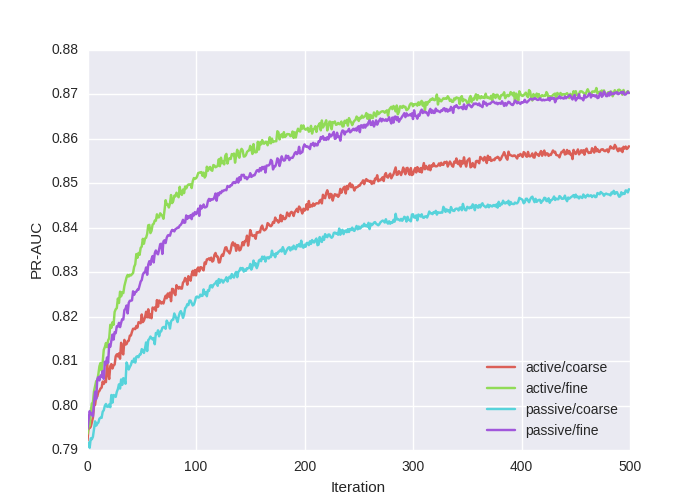
\includegraphics[width=\columnwidth]{fig/draft-interval}
		\label{fig:curve-synth}
	}\\
	\subfigure[Document classification]{
    	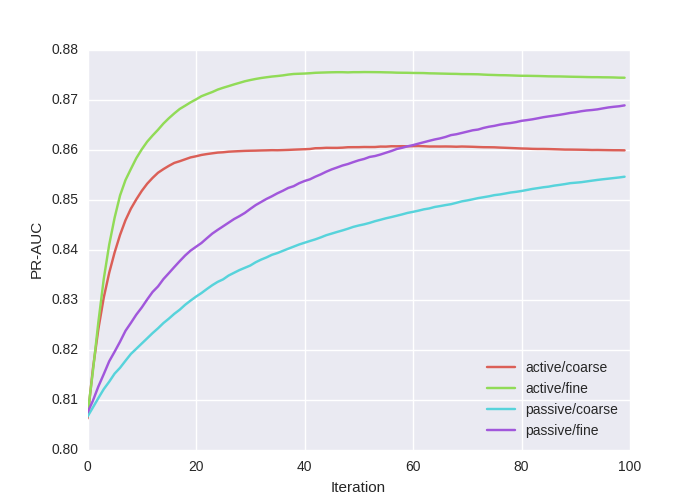
\includegraphics[width=\columnwidth]{fig/draft-RCV1}
    	\label{fig:curve-rcv1}
    }\\
    \subfigure[Sequence tagging]{
    	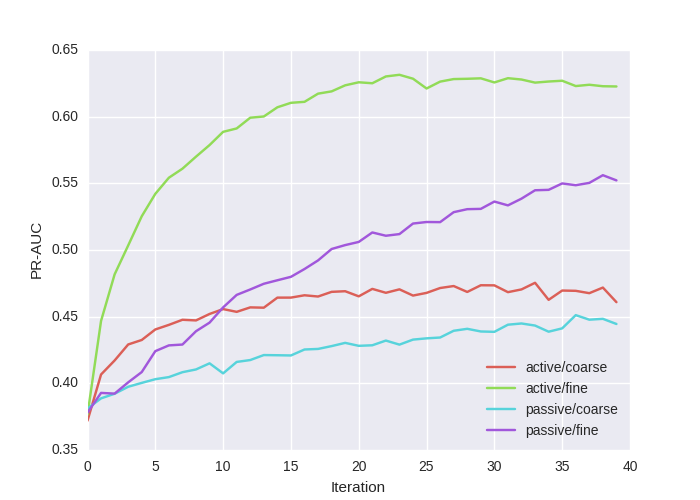
\includegraphics[width=\columnwidth]{fig/draft-richmond}
    	\label{fig:curve-richmond}
    }
    \caption{Learning curves comparing combinations of fine/coarse and active/passive PR-AUC}
  \label{fig:halresults}
\end{figure}

\subsection{Document Classification}
\label{sec:rcv1}

%We now present results from a document classification task.
The RCV1 data set~\cite{Lewis2004} contains 23,149 training documents and 781,265 test
documents labeled with a 117-node hierarchy  of Reuters Topics categories. 
Each document was represented in cosine-normalized log TF-IDF~\cite{Salton1988}
format.  Our coarse-based and fine-based learners used logistic regression~\cite{Cox1958} as
the base learner, with L2 regularization. (The regularization parameter of
$\lambda=0.1$ was chosen based on preliminary experiments; it is future work to
further tune this parameter via cross-validation.)

We used ECAT as the coarse-grained class, which contains 119,920
positive examples and 33 sub-classes in multiple levels underneath it.  
For this task we started with a seed set of 2,000 randomly-selected
instances and ran 100 iterations of active learning with 120 labels acquired
per iteration from the pool of the remaining 22,949 instances using both coarse-based and fine-based
methods. To eliminate trivially small classes,
we filtered out all fine-grained classes with fewer than 10 instances.
We tested the model on the entire test set, which is independent from the 
initial seed training set and candidate pool set. Each learning curve is the average of 50 rounds.

\subsection{Sequence Tagging}
\label{sec:richmond}

%Our third experiment focuses on entity recognition in sequences of text.  
We took OCR results from digitized editions of the {\it Richmond Daily
Dispatch} from November 1860 through December 1865 that had been
tagged with XML labels according to a two-level hierarchical labeling
scheme~\cite{RichmondDispatch}.  The dataset we used consists of
375,026 manually labelled organization names across 1,384 newspaper
articles.  These names are further categorized into a pool of 82
fine-grained categories, like bank names, railroad names and
government agency names.  Thus, the coarse-grained labels were
``organization'' versus ``not organization''
and each fine-grained label is, e.g., ``bank'' versus ``not bank''.

In the {\bf Dispatch} experiment, we used conditional random fields~(CRFs)~\cite{Sutton2006} 
as the base learner.  We trained CRFs using standard 2--3 letter prefix, postfix, capitalization and
numerical features.  We evaluate the trained CRF by performing 
the Forward-Backward algorithm~\cite{Culotta2004}
on a new sentence $s$ to get an estimate of the probability that each token
% (word or short phrase)
$x \in s$ is an organization.  Evaluating the set of tokens above
varying thresholds on this probability yields the precision-recall
curves we use for evaluation.

We compared training fine-based classifiers
via active learning, fine-based classifiers via passive learning,
coarse-based via active learning, and coarse-based via passive
learning.  First, we set aside 20,000 sentences for the test
set and 10,000 sentences for candidate set.
The experiment starts with a initial training set of 1,600 sentences.
For this task our experiments proceeded in 40 iterations, with batch sizes of
100 sentences each iteration. When computing the uncertainty of a sentence $s$,
we took the maximum uncertainty across all tokens in $s$.

\subsection{Results on active over-labeling}

For each of the three tasks described above, we built four learning curves.
The experiments compare four settings, for the four combinations of {\em active} vs. {\em passive}
learning,\footnote{Our passive learners
are trained with the same number of training instances as our active learners, but the
instances are chosen randomly rather than via uncertainty sampling.} and standard labeling vs. over-labeling with \sys .  Because standard learning
solicits coarse-grained labels for the coarse-grained task, we refer to that setting as {\em coarse}.
The coarse algorithms are representative of the state of the art in the document classification
and sequence tagging.  \sys\ uses finer-grained labels, so we refer to the over-labeling
setting as {\em fine}.

The results appear in Figure \ref{fig:halresults}.  As all three figures show, active over-labeling with
{\em active fine} is the best method across all three data sets.  These results show
how \sys\ improves accuracy by querying for examples at a finer granularity than 
that targeted for classification.

\subsection{Results as cost varies}
\label{sec:cost-sens}

The above results demonstrate the advantages offered by purchasing
fine-grained labels in an active learning context to improve performance.
So far, we have ignored differences in cost
between label types.  As discussed above, in practice fine-grained labels are likely to be
more expensive to obtain than coarse-grained labels, which means we might not be able to afford to
purchase purely fine-grained labels.

We first provide an analysis indicating that active over-labeling
is likely to provide value at varying ratios of cost between coarse and
fine-grained labels. We examine the learning curve of varying fixed ratio of
instances labeled at the fine and coarse levels in the experiments (FFR). For example,
in a setting of fine cost 16 and iteration budget of 32, FFR[0.5] allocates each of its 50\%
budget to coarse and fine, which corresponds to picking 16 coarse instances and 1 fine instance per iteration.
This curve will give us an estimate of what ratio of cost of fine-grained labels to coarse-grained
labels justifies the use of an active over-labeling approach.

\begin{figure}[tb]
	\centering
	\subfigure[Synthetic dataset]{
		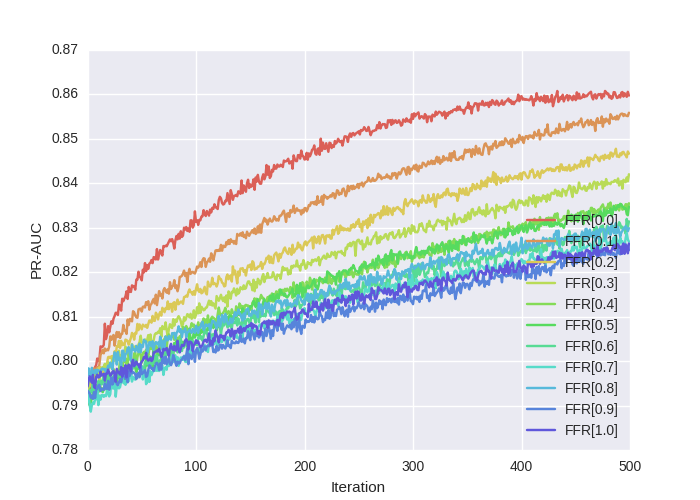
\includegraphics[width=\columnwidth]{fig/interval-16-nobandit}
		\label{fig:interval-cost16}
	}\\
	\subfigure[Document classification]{
    	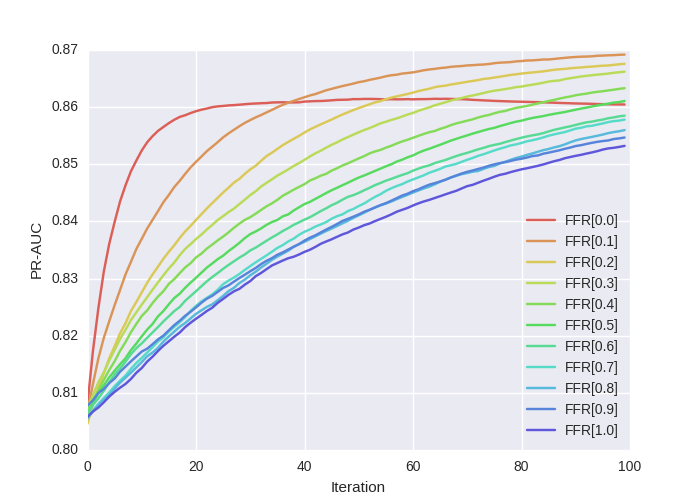
\includegraphics[width=\columnwidth]{fig/RCV1-16-nobandit}
    	\label{fig:RCV1-cost16}
    }\\
    \subfigure[Sequence tagging]{
    	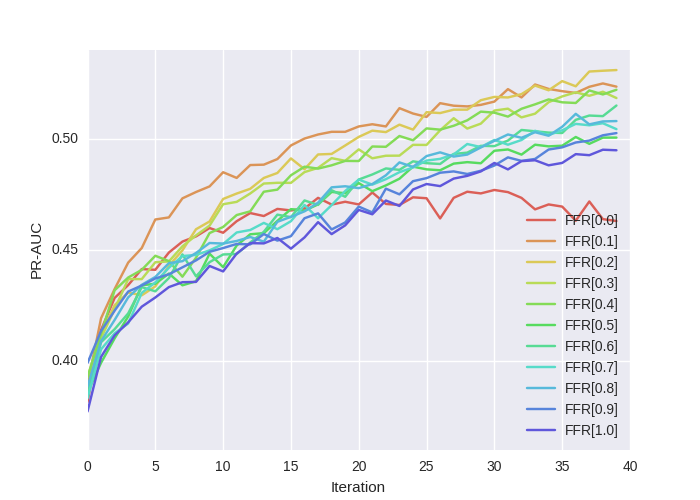
\includegraphics[width=\columnwidth]{fig/richmond-16-nobandit}
    	\label{fig:richmond-cost16}
    }
    \caption{Learning curves comparing active FFR method PR-AUC on fine cost 16}
	\label{fig:cost16}
\end{figure}

We switch from the fixed number of purchases per iteration to a fixed budget per iteration,
re-run the three experiments from Section~\ref{sec:synth}--Section~\ref{sec:richmond}, and then
compare the AUC scores achieved for active FFR learners in across experiments.

In Figure~\ref{fig:interval-cost16}, the synthetic dataset experiment, lower FFR
achieves better AUC in all $500$ iterations. The synthetic problem is easy to learn
which means the benefit of fine-grained labels cannot compensate for a fine cost as high as 16.
It is more cost effective to use a pure coarse-based classifier and not utilize fine-grained labels
at all.

In Figure~\ref{fig:RCV1-cost16}, the document classification experiment, FFR[0.0] rises fast
but quickly reaches a bottleneck, which is surpassed by FFR[0.1] in a later iteration. This problem
is less easy to learn and fine-grained labels may be worth their cost, depending on the overall budget.
If the budget is limited to fewer than 38 rounds, FFR[0.0] is the best choice; otherwise,
FFR[0.1] delivers better value than FFR[0.0].

\clearpage

In Figure~\ref{fig:richmond-cost16}, the sequence tagging experiment, the problem is harder,
so FFR[0.1]
has higher AUC than FFR[0.0] starting from the beginning. Then FFR[0.2] catches up after round 35. Higher FFR ratio
is more affordable in the long run. If the budget is less than 35 rounds then FFR[0.1] is preferred over FFR[0.2].

From Figure~\ref{fig:cost16}, we can see that the choice of FFR to achieve high AUC depends on multiple factors,
like the overall budget (the number rounds of iterations before termination), the cost of fine-grained labels and
the nature of the problem target itself.

\subsection{Results with BANDIT}

We now turn to evaluating BANDIT, which chooses purchase proportions dynamically.  We configure the two strategies
that BANDIT selects between to be the all-coarse (FFR[0.0]) and all-fine (FFR[1.0]) strategies.
We again set aside 20,000, 4,000 and 10,000 unlabeled examples for the synthetic task, document classification, 
and sequence tagging, and re-run the experiment in Section~\ref{sec:cost-sens} with
BANDIT. To evaluate the robustness of the algorithm, we test each approach for fine-grain cost varying within 
$\{1.0, 1.1, 1.2, 1.5, 2.0, 4.0, 8.0, 16.0, 32.0, 64.0\}$.


\begin{figure}[tb]
	\centering
	\subfigure[Synthetic dataset experiment]{
		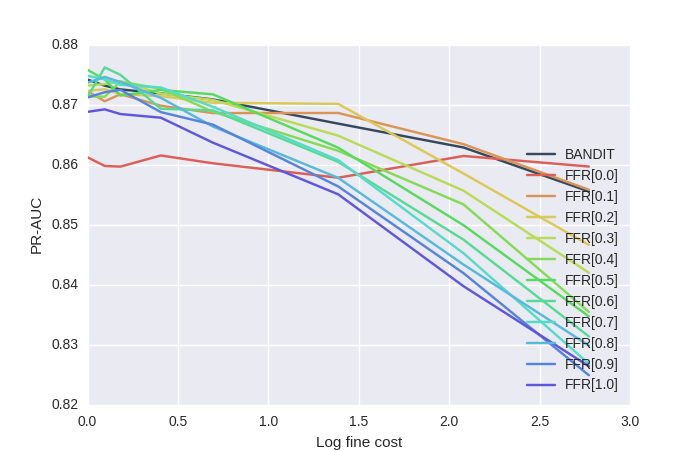
\includegraphics[width=\columnwidth]{fig/curve-interval}
		\label{fig:interval-curve}
	}\\
	\subfigure[Document classification experiment]{
    	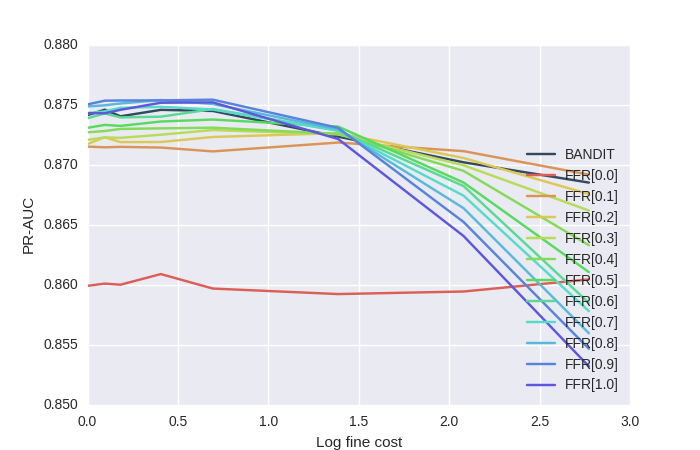
\includegraphics[width=\columnwidth]{fig/curve-RCV1}
    	\label{fig:RCV1-curve}
    }\\
    \subfigure[Sequence tagging experiment]{
    	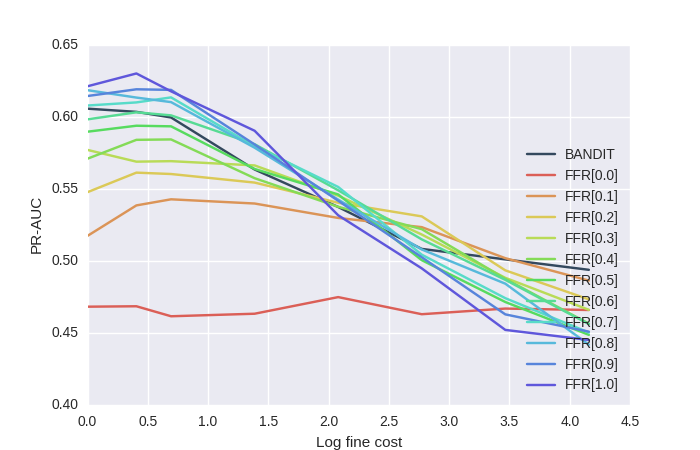
\includegraphics[width=\columnwidth]{fig/curve-richmond}
    	\label{fig:richmond-curve}
    }
    \caption{Comparing active FFR and BANDIT method PR-AUC on different fine cost}
	\label{fig:curve}
\end{figure}

Figure~\ref{fig:curve} shows the AUC for FFR and BANDIT in the end. We see that AUC in 
FFR[0.0] is not affected by the fine cost. And the AUCs for the other fixed ratio methods
FFR[0.1]-FFR[1.0] decrease as fine grained labels become more expensive, because that results in these methods 
acquiring fewer labels.
FFR with a lower fine-grained ratio achieves higher AUC when fine cost is high, and vice vesa. But the BANDIT curve is almost
always among the top curves, regardless of the fine cost. This shows how BANDIT is robust to changes in cost.

Tables~\ref{tb:synth}--\ref{tb:richmond} quantify
the observations in Figure~\ref{fig:curve}, by measuring
how close each learner is to the top-scoring learner as fine cost varies. 
The metric {\em diff} gives the learner's absolute difference from the top learner. The {\em rank} metric is
the learner's relative rank ordered by AUC.  We caculate the minimum, maximum, mean and standard deviation
for both metrics. In Table~\ref{tb:synth}, the diff of BANDIT is in the range of [0.001, 0.004] and averages
0.002 away from the top curve. and the rank of BANDIT ranges from 1 to 5 and averages 2.625.
BANDIT's mean for diff and rank is the lowest among all learners, and it has a low standard deviation, indicating
that BANDIT scores close to the top curve most of the time. 
Similar results are shown in Table~\ref{tb:RCV1} and Table~\ref{tb:richmond}, where the mean
diff of BANDIT is the lowest and the mean rank is the second lowest (as highlighted). These results illustrate
that BANDIT successfully tunes the fine-grained ratio  to cope with variable cost/benefit settings,
which is important in real-world settings where the costs and benefits from querying at different levels of granualrity
are not known in advance.

Finally, we examine how BANDIT performs as budget changes. Figure~\ref{fig:costmixed} shows the learning curves
of how AUC increases for FFR and BANDIT, averaging over different costs. On different tasks, different fine-grained
ratios may be preferable for different budgets---e.g., FFR[0.0] performs best for the first few purchases in Figure~\ref{fig:RCV1-costmixed}, but
is much worse for larger budgets.  However, in all figures, BANDIT almost always maintains the top AUC score
after the first few rounds. Thus, we expect BANDIT to perform well against fixed ratio methods across a variety of budgets.

\begin{table}[htb]
\caption{Aggregated PR AUC for synthetic dataset}
\centering
\resizebox{0.9\columnwidth}{!}{%
\begin{tabular}{lrrrrrrrr}
\hline
{} &  diff &       &       &       & rank &     &        &       \\
{} &   min &   max &  mean &   std &  min & max &   mean &   std \\
\hline
algorithm &       &       &       &       &      &     &        &       \\
BANDIT    & 0.001 & 0.004 & \underline{\textbf{0.002}} & 0.001 &    1 &   5 &  \underline{\textbf{2.625}} & 1.598 \\
FFR[0.0]  & 0.000 & 0.016 & 0.010 & 0.006 &    0 &  11 &  8.125 & 4.549 \\
FFR[0.1]  & 0.000 & 0.006 & 0.003 & 0.002 &    0 &   9 &  4.875 & 3.603 \\
FFR[0.2]  & 0.000 & 0.013 & 0.004 & 0.004 &    0 &   7 &  4.000 & 2.204 \\
FFR[0.3]  & 0.001 & 0.018 & 0.005 & 0.006 &    1 &   4 &  3.250 & 1.165 \\
FFR[0.4]  & 0.000 & 0.024 & 0.007 & 0.008 &    1 &   8 &  4.875 & 2.357 \\
FFR[0.5]  & 0.000 & 0.025 & 0.006 & 0.009 &    0 &   9 &  3.750 & 3.151 \\
FFR[0.6]  & 0.000 & 0.028 & 0.008 & 0.010 &    0 &   8 &  5.250 & 3.370 \\
FFR[0.7]  & 0.000 & 0.033 & 0.008 & 0.012 &    0 &   9 &  4.250 & 3.240 \\
FFR[0.8]  & 0.001 & 0.030 & 0.009 & 0.011 &    1 &   9 &  6.000 & 3.251 \\
FFR[0.9]  & 0.002 & 0.035 & 0.011 & 0.012 &    6 &  11 &  8.750 & 1.669 \\
FFR[1.0]  & 0.005 & 0.033 & 0.013 & 0.010 &   10 &  11 & 10.250 & 0.463 \\
\hline
\end{tabular}}
\label{tb:synth}
\end{table}

\begin{table}[htb]
\caption{Aggregated PR AUC for document classification}
\centering
\resizebox{0.9\columnwidth}{!}{%
\begin{tabular}{lrrrrrrrr}
\hline
{} &  diff &       &       &       & rank &     &        &       \\
{} &   min &   max &  mean &   std &  min & max &   mean &   std \\
\hline
algorithm &       &       &       &       &      &     &        &       \\
BANDIT    & 0.001 & 0.001 & \underline{\textbf{0.001}} & 0.000 &    1 &   8 &  3.750 & 2.188 \\
FFR[0.0]  & 0.009 & 0.016 & 0.014 & 0.002 &    6 &  11 & 10.375 & 1.768 \\
FFR[0.1]  & 0.000 & 0.004 & 0.003 & 0.002 &    0 &  10 &  7.500 & 4.629 \\
FFR[0.2]  & 0.001 & 0.004 & 0.002 & 0.001 &    1 &   9 &  6.500 & 3.381 \\
FFR[0.3]  & 0.001 & 0.003 & 0.002 & 0.001 &    3 &   9 &  6.750 & 2.375 \\
FFR[0.4]  & 0.001 & 0.006 & 0.003 & 0.002 &    4 &   7 &  6.125 & 1.356 \\
FFR[0.5]  & 0.000 & 0.008 & 0.003 & 0.002 &    0 &   6 &  5.000 & 2.070 \\
FFR[0.6]  & 0.000 & 0.011 & 0.002 & 0.003 &    3 &   7 &  4.875 & 1.356 \\
FFR[0.7]  & 0.000 & 0.011 & 0.002 & 0.004 &    2 &   8 &  4.250 & 2.121 \\
FFR[0.8]  & 0.000 & 0.013 & 0.002 & 0.005 &    0 &   9 &  3.000 & 3.464 \\
FFR[0.9]  & 0.000 & 0.015 & 0.003 & 0.005 &    0 &  10 &  \underline{\textbf{2.625}} & 4.274 \\
FFR[1.0]  & 0.000 & 0.016 & 0.003 & 0.006 &    1 &  11 &  5.250 & 4.062 \\
\hline
\label{tb:RCV1}
\end{tabular}}
\end{table}

\vspace{-0.1in}

\begin{table}[htb]
\caption{Aggregated PR AUC for sequence tagging}
\centering
\resizebox{0.9\columnwidth}{!}{%
\begin{tabular}{lrrrrrrrr}
\hline
{} &  diff &       &       &       & rank &     &       &       \\
{} &   min &   max &  mean &   std &  min & max &  mean &   std \\
\hline
algorithm &       &       &       &       &      &     &       &       \\
BANDIT    & 0.000 & 0.027 & \underline{\textbf{0.016}} & 0.011 &    0 &   8 & 4.250 & 2.712 \\
FFR[0.0]  & 0.028 & 0.162 & 0.101 & 0.056 &    4 &  11 & 9.875 & 2.475 \\
FFR[0.1]  & 0.000 & 0.104 & 0.045 & 0.041 &    0 &  10 & 6.500 & 4.840 \\
FFR[0.2]  & 0.000 & 0.074 & 0.035 & 0.029 &    0 &   9 & 5.750 & 3.845 \\
FFR[0.3]  & 0.006 & 0.061 & 0.030 & 0.020 &    3 &   8 & 5.000 & 2.330 \\
FFR[0.4]  & 0.009 & 0.050 & 0.030 & 0.016 &    2 &   8 & 6.000 & 2.138 \\
FFR[0.5]  & 0.005 & 0.045 & 0.029 & 0.011 &    2 &   9 & 6.500 & 2.268 \\
FFR[0.6]  & 0.002 & 0.038 & 0.019 & 0.011 &    1 &   6 & \underline{\textbf{3.875}} & 1.885 \\
FFR[0.7]  & 0.000 & 0.044 & 0.018 & 0.014 &    0 &   8 & 4.125 & 2.850 \\
FFR[0.8]  & 0.003 & 0.052 & 0.018 & 0.015 &    1 &  11 & 4.625 & 3.114 \\
FFR[0.9]  & 0.000 & 0.043 & 0.018 & 0.016 &    0 &  10 & 4.375 & 3.662 \\
FFR[1.0]  & 0.000 & 0.050 & 0.019 & 0.022 &    0 &  11 & 5.125 & 5.249 \\
\hline
\label{tb:richmond}
\end{tabular}}
\end{table}

\begin{figure}[tb]
	\centering
	\subfigure[Synthetic dataset experiment]{
		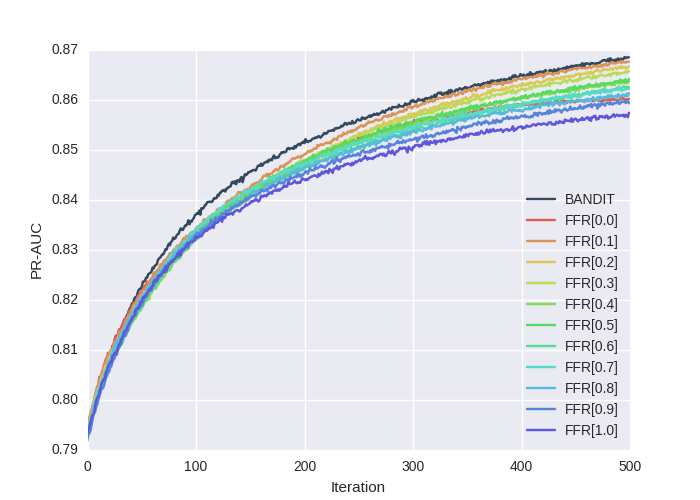
\includegraphics[width=\columnwidth]{fig/interval-mixed-bandit}
		\label{fig:interval-costmixed} 
	}\\
	\subfigure[Document classification experiment]{
    	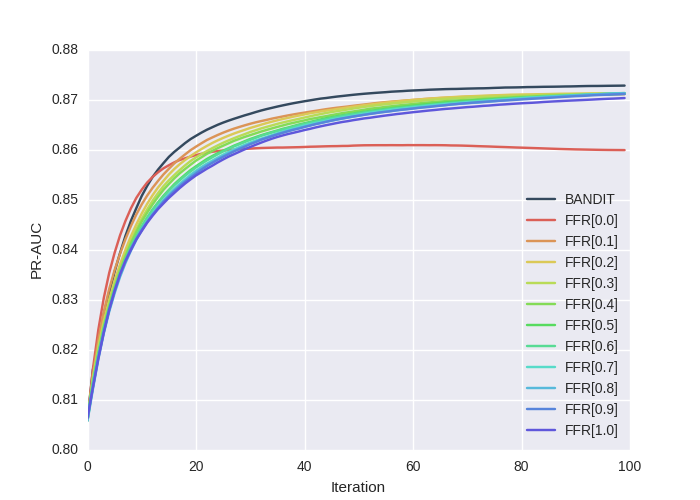
\includegraphics[width=\columnwidth]{fig/RCV1-mixed-bandit}
    	\label{fig:RCV1-costmixed}
    }\\
    \subfigure[Sequence tagging experiment]{
    	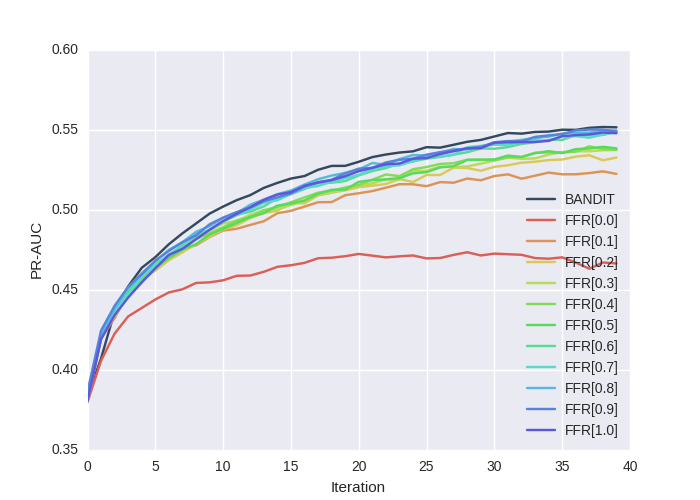
\includegraphics[width=\columnwidth]{fig/richmond-mixed-bandit}
    	\label{fig:richmond-costmixed}
    }
    \caption{Learning curves comparing active FFR and BANDIT method PR-AUC on mixed fine cost}
	\label{fig:costmixed}
\end{figure}

